%!TEX root = ../thesis.tex

\chapter{MHD Verification and Case-Specific Validation Results}
\label{chap:mhd-validation-results}

\section{Verification and validation hierarchy}
\label{sec:ch4-validation-hierarchy}

Chapter~3 defines the reference hierarchy and the checks and diagnostics used
here; each result below is conditional on its solver, precision, device, grid
and final time.

\section{Brio--Wu numerical-reference assessment}
\label{sec:ch4-brio-wu}

Figure~\ref{fig:ch4-brio-refinement} compares three fp64 grids of the coplanar
MHD Riemann problem of \citet{brioWu1988} against an $N=8000$ numerical
comparator, conservatively downsampled by averaging the $8000/N$ fine cells in
each candidate cell. From $N=200$ to $N=800$ the density mean $L_1$
difference fell monotonically from $1.481\times10^{-2}$ to
$5.642\times10^{-3}$ and $L_2$ from $3.642\times10^{-2}$ to
$1.923\times10^{-2}$, with finite states and
$\mathrm{divB}_{\max}\leq4.441\times10^{-14}$ on all three grids.
Least-squares fits of $\log_2 E = a-q\log_2 N$ give rates $q=0.70$ in $L_1$ and
0.46 in $L_2$.

Plausibly the limiter reduces formal second-order accuracy to first order near
extrema and discontinuities \citep{toro2009riemann}: at a linearly degenerate
contact a monotone scheme of order $p$ converges in $L_1$ as $h^{p/(p+1)}$, so
$p=2$ gives $h^{2/3}\approx0.67$, close to 0.70, with the lower $L_2$ rate
following from that norm weighting the smeared jump more heavily. The compound
wave and the comparator's shared discretisation bias also admit
pseudo-convergence \citep{torrilhon2003pseudo}, so the rates measure
self-consistency on these grids.

\begin{figure}[htbp]
\centering

\includegraphics[width=0.82\textwidth,viewport=0 0 260 200,clip]{Figs/report2/ch4_validation_refinement_glm}
\caption[Brio--Wu refinement]{\textbf{Brio--Wu refinement.} Density mean
$L_1$ and $L_2$ differences against the conservatively downsampled
$N=8000$ fp64 numerical comparator.}
\label{fig:ch4-brio-refinement}
\end{figure}

The $N=800$ profiles in Figure~\ref{fig:ch4-brio-profiles} visually reproduce
the sequence reported by \citet{brioWu1988}: left-going fast rarefaction, slow
compound wave, contact discontinuity, slow shock, and right-going fast
rarefaction. The contact and the slow shock are nonetheless visibly displaced
and smeared against the comparator, where the mean $L_1$ difference is
concentrated.

\begin{figure}[htbp]
\centering

\includegraphics[width=\textwidth]{Figs/report2/ch4_brio_wu_profiles}
\caption[Brio--Wu final-state profiles]{\textbf{Brio--Wu final-state profiles.}
HLL fp64 density, normal velocity, transverse magnetic field and pressure at
$t=0.1$: $N=800$ candidate and same-HLL $N=8000$ numerical comparator.}
\label{fig:ch4-brio-profiles}
\end{figure}

\section{Two-dimensional property verification and divergence control}
\label{sec:ch4-invariance-glm}

An $800\times4$ embedding of Brio--Wu tested whether the two-dimensional
update preserved a transversely constant state. The maximum transverse
deviation was zero, every row identical component by component. Against the
corresponding one-dimensional run, the mean and maximum absolute density
differences were $3.550\times10^{-4}$ and $7.034\times10^{-3}$, below the
predeclared thresholds $10^{-3}$ and $10^{-2}$. Including the $y$-direction
fast speed, the two-dimensional speed estimate required 861 rather than 759
steps; that time-step difference explains the non-zero density differences
without contradicting exact row invariance.

Figure~\ref{fig:ch4-glm-divergence} reports the Generalised Lagrange Multiplier
(GLM) diagnostic of \citet{dedner2002glm} for the doubly-periodic $128^2$ unit
square, HLL, fp64, $\gamma=2$, CFL 0.4, with $\rho=p=1$, $\mathbf{v}=0$ and all
field components zero except a Gaussian normal-field bump
$B_x=B_0\exp(-r^2/\sigma^2)$, $B_0=1$, $\sigma=0.1$, at $(0.5,0.5)$. Its
$x$-dependent $B_x$ makes the initial state non-solenoidal by construction, a
controlled test of the cleaning in which divergence is of order unity, and
each plotted stopping time is a separately executed run rather than a time
series. Here $c_r=0$ is a supported undamped control: a guard skips damping,
so no division by zero occurs. At $t=0.5$,
$\max|\nabla\!\cdot\!\mathbf{B}|$ was 3.030 for this control, 0.2678 for
$c_r=0.18$ and 0.8429 for $c_r=0.36$. Since the exponential damping
rate is $c_h/c_r$, $c_r=0.18$ damps more strongly than $c_r=0.36$, consistent
with its smaller terminal maximum.

% Source PDF SHA-256:
% ca1c0d20572818a015eb394aa3bb43786b874ce4604e889fb310f5ec4e15c442
\begin{figure}[htbp]
\centering

\includegraphics[width=0.82\textwidth,viewport=266.072 0 532.144 200,clip]{Figs/report2/ch4_validation_refinement_glm}
\caption[GLM divergence diagnostic]{\textbf{GLM divergence diagnostic.}
Maximum divergence for the doubly-periodic $128^2$ Gaussian normal-field bump
(HLL, fp64, CFL 0.4), one run per stopping time; $c_r=0$ is the undamped
control.}
\label{fig:ch4-glm-divergence}
\end{figure}

\section{Matched CPU/GPU implementation verification}
\label{sec:ch4-cpu-gpu-validation}

Case, grid, precision, arithmetic and update order were matched across separate
CPU and CUDA HLL implementations. Table~\ref{tab:ch4-cpu-gpu} reports four
pairs, Brio--Wu at $800\times1$ and Orszag--Tang at $256^2$ in fp32 and fp64,
each repeated five times, all giving zero maximum ULP and zero absolute
$L_\infty$ difference. The $c_h$ reduction was reordered from a sequential CPU
scan into a parallel GPU maximum tree, which cannot accumulate rounding, and
device contraction was disabled to match the host
(Section~\ref{sec:ch2-execution}); the agreement holds for that build recipe. A
shared defect would still agree bit for bit.

% Generated by scripts/figures/report2_chapter4_cpu_gpu_table.py
% Source: experiments/week16/cpu_gpu_hardware_axis/summary.json
\begin{table}[htbp]
\centering
\small
\begin{tabularx}{\textwidth}{@{}llccccX@{}}
\toprule
Case & Precision & Grid & CPU/GPU steps & $\mathrm{ULP}_{\max}$ & $L_\infty$ & Verified output \\
\midrule \addlinespace[2pt]
Brio--Wu & fp64 & $800\times1$ & 759/759 & 0 & 0 & HLL saved state \\
Brio--Wu & fp32 & $800\times1$ & 759/759 & 0 & 0 & HLL saved state \\
Orszag--Tang & fp64 & $256^2$ & 806/806 & 0 & 0 & HLL saved state \\
Orszag--Tang & fp32 & $256^2$ & 806/806 & 0 & 0 & HLL saved state \\
\bottomrule
\end{tabularx}
\caption[Matched CPU/GPU MHD implementation verification]{\textbf{Matched CPU/GPU MHD implementation verification.} Same-precision CPU and GPU HLL runs used the same case configuration on the recorded workstation. Steps are reported as CPU/GPU, and $L_\infty$ denotes the absolute difference between saved states. All four comparisons are bit-identical.}
\label{tab:ch4-cpu-gpu}
\end{table}


\section{Orszag--Tang validation}
\label{sec:ch4-orszag-tang}

The Orszag--Tang test uses the periodic unit-square rescaling of
\citet{toth2000divb}. The HLL runs at $128^2$, $256^2$, and $512^2$ completed
with finite, positive physical states. Under refinement the mean divergence
diagnostic fell from 0.1364 to 0.1036 while its local maximum rose from 1.734
to 7.729. Both are dimensional, so the ladder is better read in grid
units \citep{toth2000divb}. Scaled by the cell width the domain mean falls
about fivefold, $1.07\times10^{-3}$, $4.79\times10^{-4}$,
$2.02\times10^{-4}$, so cleaning works wherever the field is smooth, while the
maximum barely moves, 0.0136, 0.0145 and 0.0151, roughly $1.4\%$ of $B_0$ per
cell width. Without explicit resistivity, ideal MHD current sheets keep
thinning under refinement, leaving a sheet a few cells across whose
central-difference residual scales as $1/h$, so the peak stays pinned at the
grid scale and the raw growth reflects the diagnostic's dimensions, not lost
divergence control. The audited fp64 HLL $256^2$--$512^2$ pair also retained zero relative mass drift,
and its temperature field preserved the interacting-shock and current-sheet
topology of published calculations
\citep{toth2000divb,bardDorelli2014gpu} (Figure~\ref{fig:ch4-ot-morphology}).

\begin{figure}[htbp]
\centering

\includegraphics[width=\textwidth]{Figs/report2/ch4_orszag_tang_morphology}
\caption[Orszag--Tang temperature morphology]{\textbf{Orszag--Tang temperature
morphology.} HLL fp64 temperature at $256^2$ and the internal higher-resolution
$512^2$ HLL comparator at $t=0.5$, plotted on one scale.}
\label{fig:ch4-ot-morphology}
\end{figure}

Figure~\ref{fig:ch4-resolution-precision} gives the adjacent-grid diagnostic
$p=\log_2(E_{\mathrm{coarse}}/E_{\mathrm{fine}})$, with $E$ the density
mean-$L_1$ difference between successive grids, so $p=1$ if that difference
halves on each doubling and $p=2$ if it quarters. The two-dimensional update
composes its sweeps as a fixed $x$-then-$y$ Lie splitting, which is first order
as a multidimensional split (Section~\ref{sec:ch2-mhd-glm}), so the reference
here is $p\simeq1$ rather than 2, and minmod limiting lowers it further
wherever it activates. For fp64 HLL, the differences were 0.1203 and 0.07722,
giving $p\simeq0.639$; for HLLD \citep{miyoshiKusano2005hlld}, 0.07515 and
0.04182, giving $p\simeq0.846$. Both fall below that reference, as shocks and
current sheets holding the limiter active across much of the domain would
produce; neither value is anomalous, and neither reaches even the
splitting-limited rate. Their ordering is not a solver comparison, since the
two ladders ran at CFL 0.4 and 0.2 respectively. The fp32 values agreed at the
displayed precision.

The canonical case CFL is 0.4; only the HLLD resolution ladder used 0.2. An
exploratory fp64 HLLD run at $512^2$ terminated with diagnosed negative
pressure at CFL 0.4 and again at 0.2, so reducing the time step was not the fix.
Pressure is recovered as
$p=(\gamma-1)[E-\rho|\mathbf{v}|^2/2-|\mathbf{B}|^2/2]$, so where magnetic and
kinetic energy dominate $E$ the subtraction cancels leading digits and the
relative error in $p$ is amplified by roughly $E/p$
\citep{higham2002accuracy}. The guard therefore detects a
cancellation-sensitive recovery; whether the failure threshold depends on the
working precision was not tested.
With the per-line first-order HLL fallback enabled, the HLLD ladder completed
at $128^2$, $256^2$, and $512^2$ using CFL 0.2. The code carries no
fallback-activation counter, so how much of that ladder was evaluated with
first-order HLL fluxes is unknown, and its $512^2$ diagnostics describe the
solver together with its fallback policy rather than HLLD alone. The
Kelvin--Helmholtz ladder inherited 0.2 mechanically, whereas its separate CFL
sweep completed HLLD runs at 0.2, 0.4, 0.6, and 0.8
(Section~\ref{sec:ch5-thread-cfl}). Figure~\ref{fig:ch4-ot-solver-comparison}
nonetheless shows where the two $256^2$ solver fields differ relative to the
same HLL $512^2$ context.

\begin{figure}[htbp]
\centering

\includegraphics[width=\textwidth]{Figs/report2/ch4_orszag_tang_solver_comparison}
\caption[Orszag--Tang HLL/HLLD field comparison]{\textbf{Orszag--Tang
HLL/HLLD field comparison.} Left-half temperature at $t=0.5$ for fp64 HLL and
HLLD at $256^2$, with the internal HLL $512^2$ field as refinement context.}
\label{fig:ch4-ot-solver-comparison}
\end{figure}

% Source PDF SHA-256:
% 36c516bdd93a30a13861430752bd7b7f732f1f12b91253ae616fc59b8850c017
\begin{figure}[htbp]
\centering
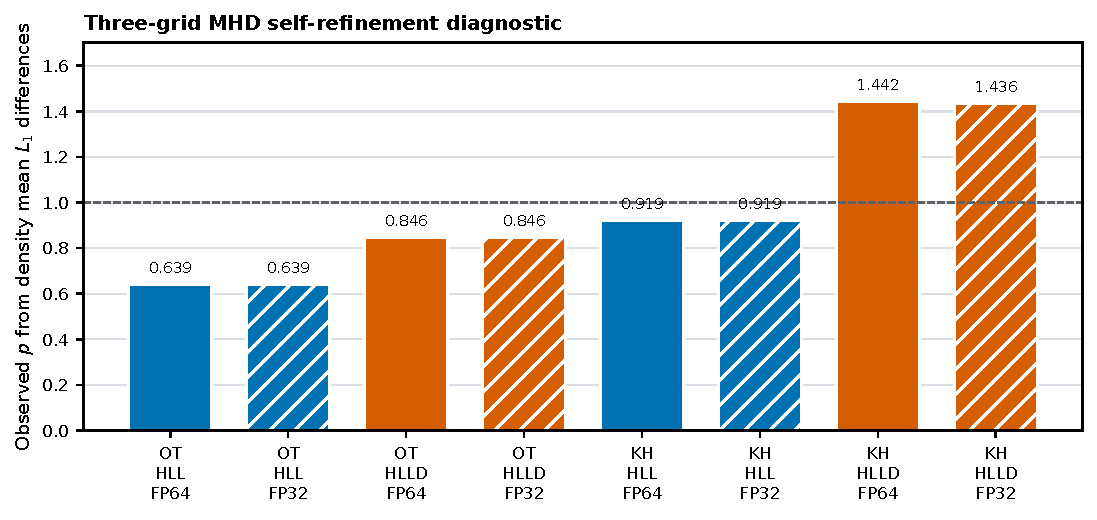
\includegraphics[width=\textwidth]{Figs/report2/ch4_resolution_precision}
\caption[Three-grid MHD resolution diagnostics]{\textbf{Three-grid MHD
resolution diagnostics.} Adjacent grids are conservatively block-averaged
before the density mean $L_1$ difference is formed. HLL uses CFL 0.4 and HLLD
uses CFL 0.2. The dashed line marks $p=1$, the first-order behaviour expected
from the fixed directional splitting: bars near it are splitting-limited, bars
below it lose further order where limiting is active.}
\label{fig:ch4-resolution-precision}
\end{figure}

\section{Kelvin--Helmholtz validation}
\label{sec:ch4-kelvin-helmholtz}

The initial data (Equation~\ref{eq:ch3-ic-kh}) for this periodic MHD problem
are a smooth double shear layer of width $a=0.025$, a shear jump of $2U_0=1$
across each layer, a single-wavelength $\sin(2\pi x)$ seed, and a uniform
flow-aligned field $B_x=0.1$, giving an Alfv\'en Mach number of 5. In the
regime of \citet{frankEtAl1996kh}, such a weak aligned field cannot suppress
the instability, though it can modify the nonlinear stage. At a sonic Mach
number of about 0.39 the case is subsonic and only weakly compressible, so
density is a low-contrast diagnostic here. That seed admits one structure on
each shear layer, with which Figure~\ref{fig:ch4-kh-morphology} is consistent
without establishing it. The sensitive variables, transverse velocity and
magnetic energy, were not measured, and the smooth-initial-condition linear
growth rates of \citet{berlokPfrommer2019kh} are the quantitative check this
report did not perform.

All solver--precision groups completed at $128^2$, $256^2$, and $512^2$ with
finite, positive states. For fp64 HLL, the mean divergence diagnostic fell
from $6.877\times10^{-5}$ to $2.305\times10^{-5}$ while the raw maximum rose
from $6.029\times10^{-4}$ to $9.236\times10^{-4}$; HLLD's raw mean and maximum
fell, from $2.747\times10^{-4}$ to $3.479\times10^{-5}$ and $9.023\times10^{-3}$
to $5.149\times10^{-3}$. Scaled by cell width and by the uniform field
$B_0=0.1$, both maxima fall monotonically as dimensionless field errors per
cell, from $4.7\times10^{-5}$ to $1.8\times10^{-5}$ for HLL and from
$7.1\times10^{-4}$ to $1.0\times10^{-4}$ for HLLD: two to three orders of
magnitude tighter than Orszag--Tang's $1.4\%$, and tightening under refinement
rather than pinned at the grid scale. Such a residual bounds the spurious
monopole forcing the update can introduce, without showing the field itself to
be accurate. HLLD's maximum stays about an order of magnitude above HLL's;
plausibly the less dissipative solver preserves sharper gradients in
$\mathbf{B}$, which the centred-difference residual registers as a larger
constraint error, so low dissipation and tight discrete divergence control are
not obtained together. Unlike Orszag--Tang's thinning current sheets, the shear
layer keeps a fixed width $a=0.025$, about three cells at $128^2$ and thirteen
at $512^2$, so refinement resolves it and the peak leaves the grid scale. The
fp64 HLL $256^2$--$512^2$ pair also retained zero relative mass drift.

\begin{figure}[htbp]
\centering

\includegraphics[width=0.76\textwidth]{Figs/report2/ch4_kelvin_helmholtz_morphology}
\caption[Kelvin--Helmholtz density morphology]{\textbf{Kelvin--Helmholtz
density morphology.} fp64 HLL density isolines at $256^2$ and $t=1.0$ for the
project-defined weak-field double shear. The plotted density range is
$0.985744$--$1.005060$, with 24 linearly spaced levels.}
\label{fig:ch4-kh-morphology}
\end{figure}

For fp64 HLL and HLLD, the adjacent-grid density differences shrink with
$p=0.919$ and $p=1.442$, respectively. On this smooth field the HLL value sits
close to the splitting-limited reference of Section~\ref{sec:ch4-orszag-tang},
whereas the HLLD value exceeding one indicates that three grids have not
reached an asymptotic regime rather than a better-than-first-order method.
These are self-refinement rates, and
\citet{lecoanetEtAl2016kh} show why nonlinear morphology alone is not an
accuracy criterion.
Without an independent field reference these checks cannot quantify solution
error, and on three grids spanning shocks and current
sheets the leading truncation term need not dominate. Chapter~5 interprets its
discrepancies accordingly.
